\chapter{L\'evy Processes}
\label{sec:Levy}

\cleanchapterquote{Paul L\'evy was a painter in the probabilistic world.}{Michel Lo\`eve}{(1907-1979)}

L\'evy processes play a central role in mathematical finance. They can describe the reality of financial markets in a more accurate way than models based on the geometric Brownian motion used in particular in Black-Scholes model. Indeed we can observe in the real world that the asset price processes have some jumps. Moreover, the log returns of the underlying have empirical distributions with fat tails and skewness which deviate from normality supposed by Black and Scholes. We begin this chapter, in Section \ref{sec:Levy:definitions}, with the definition of a L\'evy process and expose its fundamental properties. Next, in section \ref{sec:Levy:theorems}, we present two main results about L\'evy processes, namely the L\'evy-Khinchine formula and the L\'evy-Itô decomposition. In Section \ref{sec:Levy:Levy_measure}, the L\'evy measure and  path properties of a L\'evy process are exposed. Finally, Section \ref{sec:Levy:exponential_processes} presents the class of exponential L\'evy processes and the equivalent martingale measure used to describe the asset price in financial modeling.

\section{Definitions and properties}
\label{sec:Levy:definitions}
L\'evy processes are continuous time stochastic processes used as the main ingredients for building continuous-time stochastic models. The simplest L\'evy process is the linear drift. The Wiener process, Poisson process, and compound Poisson process are the most famous examples of L\'evy processes. We will see later in this chapter that the sum of a linear drift, a Wiener process, and a compound Poisson process is again a L\'evy process. It is called a \textit{L\'evy jump-diffusion} process.

\begin{defn}[Wiener Process]\label{def:wiener}
A stochastic process $W = \{W_t,t\geq 0\}$, with $W_0=0$, is a \textbf{Wiener process}, also called a standard Brownian motion, on a probability space $(\Omega,\mathcal{F},\mathbb{P})$ if:
\begin{my_list_num}
\item $W$ has independent increments, i.e. $(W_{t+s}-W_t)$ is independent of $\mathcal{F}_t$ for any $s>0$.
\item $W$ has stationary increments, i.e. the distribution of $(W_{t+s}-W_t)$ does not depend on $t$.
\item $W$ has Gaussian increments, i.e. $(W_{t+s}-W_t) \sim \mathcal{N}(0,s)$.
\item $W$ is stochastically continuous, i.e. $$\forall \epsilon>0: \lim_{s \to t}\mathbb{P}(|W_t-W_s|>\epsilon)=0.$$
\end{my_list_num}
\end{defn}

This motion was discovered by Brown in 1827 and taken back by \citeauthor{Bac00} \citeyearpar{Bac00} \cite{Bac00} to model the stock market prices. Only in 1923 the Brownian motion was defined and constructed rigorously by R. Wiener.

\begin{defn}[Poisson process]\label{def:poisson}
Let $(\tau_i)_{i\geq 1}$ be a sequence of independent exponential random variables with parameter $\lambda$ and $T_n = \sum_{i=1}^n \tau_i$. The process $N = \{N_t,t\geq 0\}$, with $N_0=0$, defined by
$$N_t = \sum_{n\geq 1}\mathbf{1}_{\{t\geq T_n\}}$$
is called \textbf{Poisson process} with intensity $\lambda$.

This process has the following properties:
\begin{my_list_num}
\item $N$ has independent increments, i.e. $(N_{t+s}-N_t)$ is independent of $\mathcal{F}_t$ for any $s>0$. 
\item $N$ has stationary increments, i.e. the distribution of $(N_{t+s}-N_t)$ does not depend on $t$.
\item $N$ has Poisson increments, i.e. $(N_{t+s}-N_t)$ has a Poisson distribution with parameter $\lambda s$.
\item $N$ is stochastically continuous, i.e. $$\forall \epsilon>0: \lim_{s \to 0}\mathbb{P}(|N_{t+s}-N_t|>\epsilon)=0.$$
\end{my_list_num}
When the process is characterized by a constant intensity parameter $\lambda$, we say that the process is homogeneous. If the intensity parameter varies with time $t$ as $\lambda(t)$, the process is said to be non-homogeneous.
\end{defn}

The Poisson process, which bears the name of the French physicist and mathematician Sim\'eon Denis Poisson, defines a counting process. It counts the number of random times $(T_n)$ which occur in $[0,t]$. Therefore, this is an increasing pure jump process. The jumps of size 1 occur at times $T_n$ and the intervals between two jumps are exponentially distributed. If we compare definitions \ref{def:wiener} and \ref{def:poisson}, we can see that only the third property differs between the two processes, only the distribution changes. The main idea of a L\'evy process is to ignore the distribution of increments.

\begin{defn}[L\'evy process]
A cadlag stochastic process $X =\{X_t,t\geq 0\}$ on $(\Omega,\mathcal{F},\mathbb{P})$ with real values is called a \textbf{L\'evy process} if it has the following properties:
\begin{my_list_num}
\item $X$ has independent increments, i.e. $(X_{t+s}-X_t)$ is independent of $\mathcal{F}_t$ for any $s>0$. 
\item $X$ has stationary increments, i.e. the distribution of $(X_{t+s}-X_t)$ does not depend on $t$. 
\item $X$ is stochastically continuous, i.e. $$\forall \epsilon>0: \lim_{s \to 0}\mathbb{P}(|X_{t+s}-X_t|<\epsilon)=0.$$
\end{my_list_num}
\end{defn}

The third condition does not imply that the sample paths are continuous. In fact, the Brownian motion is the only (non-deterministic) L\'evy process with continuous sample paths. This condition serves to exclude jumps at non-random times. In other words, for a given $t$, the probability of seeing a jump at $t$ is zero, discontinuities occur at random time. The compound Poisson process is a good example of a L\'evy process.

\begin{defn}[Compound Poisson process]
A \textbf{compound Poisson process} with intensity $\lambda > 0$ and jump size distribution $f$ is a stochastic process $X=\{X_t,t\geq 0\}$ defined as 
$$X_t = \sum_{i=1}^{N_t}Y_i,$$
where jumps size $Y_i$ are i.i.d. with the density function $f$ and $N=\{N_t,t\geq 0\}$ is a Poisson process with intensity $\lambda$, independent from $(Y_i)_{i\geq 1}$.
\end{defn}
We can easily deduce the following properties from this definition:
\begin{my_list_num}
\item The sample paths of $X$ are cadlag piecewise constant functions.
\item The jump times $(T_i)_{i\geq 1}$ have the same law as the jump times of the Poisson process $N_t$. They can be expressed as partial sums of an independent exponential random variable with parameter $\lambda$.
\item The jump sizes $(Y_i)_{i\geq1}$ are i.i.d. with law $f$.
\end{my_list_num}
We can also see that the Poisson process itself can be seen as a compound Poisson process with $Y_i \equiv 1$. This explains the origin of the name of the definition. Finally, the compound Poisson process allows us to work with jump sizes which have an arbitrary distribution.

\section{L\'evy-Khinchine formula and L\'evy-Itô decomposition}
\label{sec:Levy:theorems}
We will now present in this section two main results about L\'evy processes: the \textit{L\'evy-Khinchine formula} and the \textit{L\'evy-Itô decomposition}. Let's start with the relationship between infinitely divisible distributions and L\'evy process.

\begin{defn}[Infinite divisibility]
A probability distribution $F$ is said to be \textbf{infinitely divisible} if for any integer $n\geq 2$, there exists $n$ i.i.d. random variables $Y_1,\ldots,Y_n$ such that $Y_1+\cdots+Y_n$ has distribution $F$.
\end{defn}
If $X$ is a L\'evy process, for any $t>0$ the distribution of $X_t$ is infinitely divisible. This comes from the fact that for any $n \geq 1$,
\begin{equation}\label{eq:inf-div}
X_t = X_{t/n} + (X_{2t/n}-X_{t/n}) + \cdots + (X_t - X_{(n-1)t/n})=nX_{t/n},
\end{equation}
and the property of stationary and independent increments. Let us define now the characteristic function and characteristic  exponent of $X_t$.

\begin{defn}[Characteristic function and exponent]\label{def:Levy:CF_CE}
The \textbf{characteristic function} $\Phi_t$ of a random variable $X_t$ with cumulative distribution $F_t$ is given by
$$\Phi_t(u) = \mathbb{E}\left[e^{iu X_t}\right]=\int_{-\infty}^{\infty}e^{iu x}dF_t(x).$$
Its \textbf{characteristic exponent} is given by
$$\Psi_t(u) = \log\left(\mathbb{E}\left[e^{iu X_t}\right]\right),$$
for $u \in\mathbb{R}$ and $t>0$.
\end{defn}

 Then using twice equation \eqref{eq:inf-div} we obtain for any positive integers $m,n$ that
$$m\Psi_1(u) = \Psi_m(u) = n \Psi_{m/n}(u).$$
Hence for any rational $t=\frac{m}{n}>0$ we have
$$\Psi_t(u) = t\Psi_1(u).$$
We can generalize this relation for all $t>0$ with the help of the almost sure continuity of $X$ and a sequence of rational $\{t_n, n\geq 1\}$ such that $t_n\downarrow t$.

In conclusion, any L\'evy process has the property that for all $t>0$
$$\mathbb{E}\left[e^{iu X_t}\right] = e^{t\Psi(u)},$$
where $\Psi(u) = \Psi_1(u)$ is the characteristic exponent of $X_1$.

Then it is clear that each L\'evy process has an infinitely divisible distribution. This allows us to apply the celebrated L\'evy-Khinchine formula. 

\begin{thm}[Lévy-Khintchine formula]\label{thm:Levy:LK}
Each L\'evy process can be characterized by a triplet $(\gamma,\sigma,\nu)$ with $\gamma \in \mathbb{R},\sigma \geq 0$ and $\nu$ a measure satisfying $\nu(\{0\}) = 0$ and
$$\int_\mathbb{R} \min\{1,|x|^2\}\nu(dx)<\infty.$$
In term of this triplet the characteristic function of the L\'evy process equals:
\begin{align}\label{eq:LK}
\Phi_t(u) &= \mathbb{E}\left[\exp(i u X_t)\right]\nonumber\\
&= \exp\left(t\left(i\gamma u -\frac{1}{2}\sigma^2u^2+\int_\mathbb{R}\left(e^{iux}-1-iux\mathbf{1}_{\{|x|<1\}}\right)\nu(dx)\right)\right).
\end{align}
\end{thm}
(The proof can be find in \citeauthor{TC03} \citeyearpar{TC03} \cite{TC03})

The triplet $(\gamma,\sigma,\nu)$ is called the \textit{L\'evy} or \textit{characteristic triplet}. Moreover, $\gamma$ is called the \textit{drift term}, $\sigma$ the \textit{Gaussian} or \textit{diffusion coefficient} and $\nu(dx)$ is the \textit{L\'evy measure}, being the intensity of jumps of size $x$. This brings us to the following great result which is the L\'evy-Itô decomposition.

\begin{thm}[L\'evy-Itô decomposition]
Consider a triplet $(\gamma,\sigma,\nu)$ where $\gamma\in\mathbb{R}$, $\sigma\geq 0$ and $\nu$ is a measure satisfying $\nu(\{0\}) = 0$ and
$$\int_\mathbb{R} \min\{1,|x|^2\}\nu(dx)<\infty.$$
Then, there exists a probability space $(\Omega,\mathcal{F},\mathbb{P})$ on which four independent L\'evy processes exist, $X^{(1)},X^{(2)},X^{(3)}$ and $X^{(4)}$, where $X^{(1)}$ is a constant drift, $X^{(2)}$ is a Wiener process, $X^{(3)}$ is a compound Poisson process and $X^{(4)}$ is a square integrable (pure jump) martingale with an a.s. countable number of jumps of magnitude less than 1 on each finite time interval. Taking $X = X^{(1)}+X^{(2)}+X^{(3)}+X^{(4)}$, we have that there exists a probability space on which a L\'evy process $X = \{X_t,0\leq t \leq T\}$ with characteristic exponent
$$\Psi(u) = i\gamma u -\frac{1}{2}\sigma^2u^2+\int_\mathbb{R}\left(e^{iux}-1-iux\mathbf{1}_{\{|x|<1\}}\right)\nu(dx),$$
for all $u\in\mathbb{R}$, is defined.
\end{thm}
(See \citeauthor{Kyp06} \citeyearpar{Kyp06} \cite{Kyp06} for the proof)


The L\'evy process is characterized by its triplet $(\gamma,\sigma,\nu)$. The simplest L\'evy process is the linear \textit{drift} with the triplet $(\gamma,0,0)$. Adding a \textit{diffusion} component we get the triplet $(\gamma,\sigma,0)$ which is the case of the Black-Scholes model. A \textit{pure jump} process will be identified by the triplet $(0,0,\nu)$ and finally a \textit{L\'evy jump-diffusion} process will have the complete triplet $(\gamma,\sigma,\nu)$. The figure~\ref{fig:Levy:examples} illustrates some examples of L\'evy processes.

\begin{figure}[!htb]
	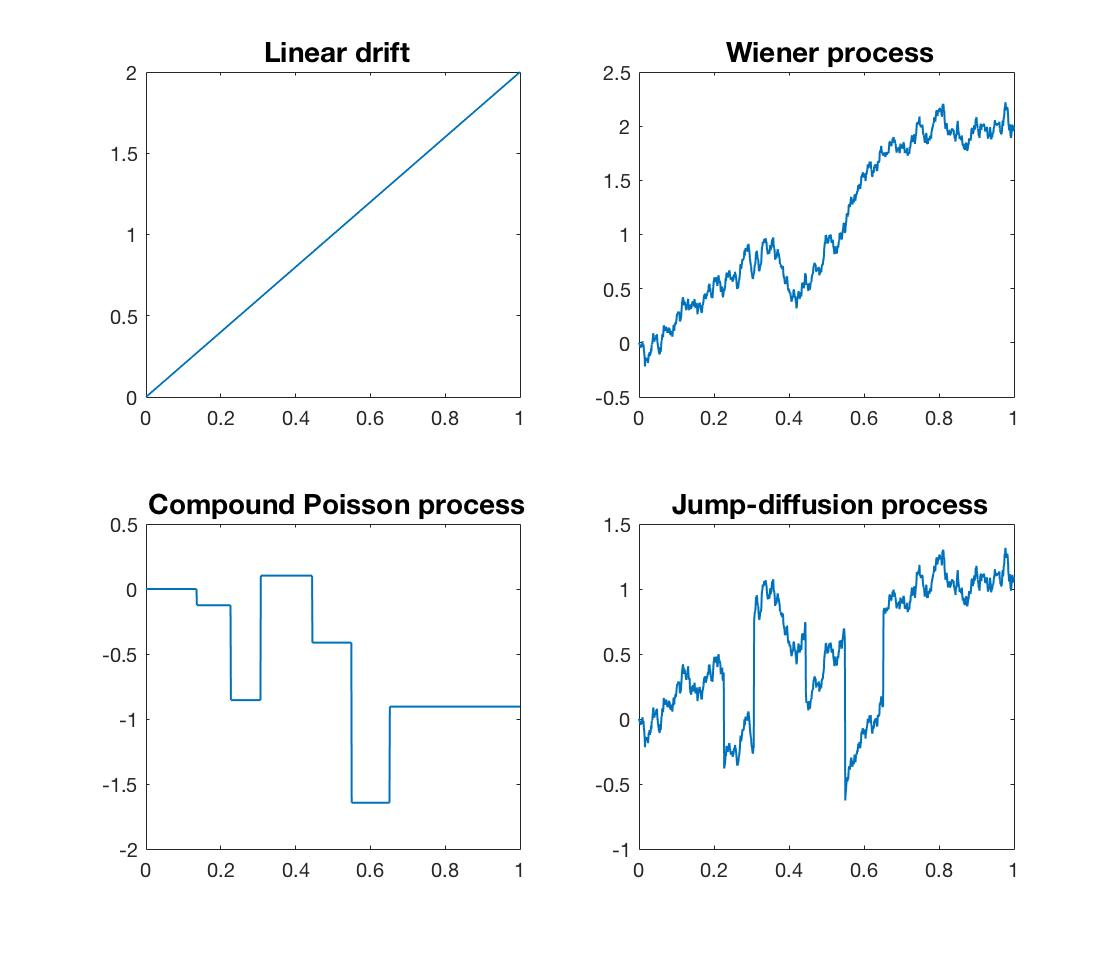
\includegraphics[width=\textwidth]{gfx/processes_examples}
	\caption{Examples of L\'evy processes: a linear drift with L\'evy triplet $(2,0,0)$, a Wiener process with L\'evy triplet $(2,1,0)$, a compound Poisson process with L\'evy triplet $(0,0,\lambda\cdot f_J)$, where $\lambda = 5$, and $f_J\sim\mathcal{N}(0,1)$ and finally a jump-diffusion process with L\'evy triplet $(2,1,\lambda\cdot f_J)$.}
	\label{fig:Levy:examples}
\end{figure}

\section{L\'evy measure and path properties}
\label{sec:Levy:Levy_measure}
The \textit{L\'evy measure} dictates the behavior of the jumps.
\begin{defn}[L\'evy measure]
Let $X = \{X_t,t\geq 0\}$ be a L\'evy process on $\mathbb{R}$. The measure $\nu$ on $\mathbb{R}$ defined by
$$\nu(A) = \mathbb{E}\left[\#\{t\in[0,1]:\Delta X_t = X_t-X_{t^-} \neq 0, \Delta X_t\in A\}\right],$$
is called the \textbf{L\'evy measure} of $X$: $\nu(A)$ is the expected number, per unit time, of jumps whose size belongs to $A$.
\end{defn}

For example, the L\'evy measure of a compound Poisson process is given by $\nu(dx) = \lambda f_J(x)dx$, where $f_J(x)$ is called the L\'evy density. In other words, the expected number of jumps, in a time interval of length 1, is $\lambda$, and the jump size is distributed according to $f_J$.

More generally, if $\nu$ is a finite measure, that is $\lambda = \nu(\mathbb{R}) =\int_\mathbb{R}\nu(dx) <\infty$, 
then we can defined $f(dx) = \frac{\nu(dx)}{\lambda}$, which is a probability measure. Then, $\lambda$ is the expected number of jumps and $f(dx)$ is the distribution of the jump size $x$. If $\nu(\mathbb{R}) = \infty$, an infinite number of (small) jumps is expected.

\begin{prop}[Finite and infinite activity]
Let $X =\{X_t,t\geq 0\}$ be a L\'evy process with triplet $(\gamma,\sigma,\nu)$.
\begin{my_list}
\item If $\nu(\mathbb{R})<\infty$ then almost all paths of $X$ have a finite number of jumps on every compact interval. In that case, the L\'evy process has \textbf{finite activity}.
\item If $\nu(\mathbb{R})=\infty$ then almost all paths of $X$ have a infinite number of jumps on every compact interval. In that case, the L\'evy process has \textbf{infinite activity}.
\end{my_list}
\end{prop}
(See Theorem 21.3 in \citeauthor{Sat99} \citeyearpar{Sat99} \cite{Sat99} for the proof)

Then the L\'evy jump models can be classified into two categories from their L\'evy measure: jump-diffusion or pure jump models. The jump-diffusions models are modeled by a Gaussian part (Wiener process) combined with a jump part (compound Poisson process), that has finitely many jumps in every time interval, i.e. finite activity models. The second category consists of models with an infinite number of jumps in every interval, i.e. infinite activity models. In these models, there is no need of Gaussian part because the dynamics of jumps is already rich enough to generate nontrivial small time behavior. Merton model and Variance Gamma model are good examples of jump-diffusion and pure jump models respectively. In Figure \ref{fig:Levy:densities} are represented their respective L\'evy densities. In Variance Gamma model, the density explodes at the origin. This means that the model allows infinitely many very small jumps. Since the L\'evy density of Merton model is continuous, there is finite number of jumps on every time interval.

\begin{figure}[!htb]
	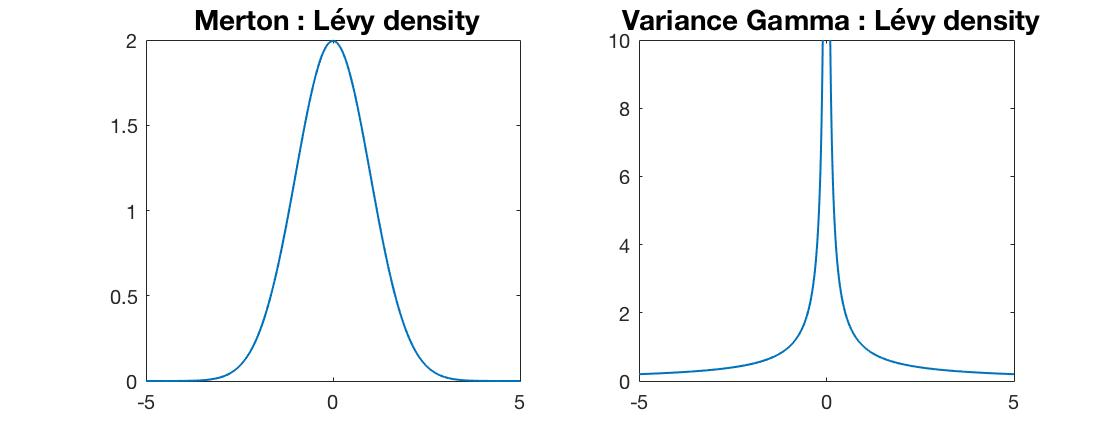
\includegraphics[width=\textwidth]{gfx/Levy_densities}
	\caption{The density of L\'evy measure in the Merton model (left) and the Variance Gamma model (right).}
	\label{fig:Levy:densities}
\end{figure}

\section{Exponential L\'evy processes and Equivalent martingale measure}
\label{sec:Levy:exponential_processes}

In finance, it is common to model the stock price process as the exponential of a L\'evy process:
$$S_t = S_0 e^{X_t}, \qquad \text{with }X_0=0.$$
The advantage of this representation is that the stock prices process is nonnegative and the log returns $\log(S_{t+s}/S_t)$, for $s,t>0,$ follow the distribution of increments of length $s$ dictated by the L\'evy process $X=\{X_t,t\geq0\}$. Thus they have independent and stationary increments.

In order to avoid an arbitrage opportunity, the discounted and reinvested process $\hat{S}=\{\hat{S}_t = e^{-(r-q)t}S_t,t\geq0\}$ has to be a martingale under an \textit{equivalent martingale measure} (EMM) $\mathbb{Q}$, called the \textit{risk-neutral measure}. Recall that $r$ is the \textit{(domestic) risk-free rate} and $q$ is the \textit{continuous dividend yield (or foreign interest rate in the FX market)} of the asset. In other words, we are looking for a measure $\mathbb{Q}$ such that
$$\mathbb{E}^\mathbb{Q}\left[\hat{S}_T|\mathcal{F}_t\right]=\hat{S_t}.$$
Since the market is not complete under L\'evy processes, there exists several ways to find a risk-neutral measure. We will see two different methods to determine this probability measure.

\subsection{Esscher transform method}
The first approach to find an EMM $\mathbb{Q}$ is proposed by \citeauthor{G+94} \citeyearpar{G+94} \cite{G+94} using the Esscher transform. Suppose that the L\'evy process $X=\{X_t,t\geq0\}$ has a density function $f(x;t)$. Now multiply this density by an exponential factor $e^{\theta t}$ to get a new density function:
$$f(x;t,\theta) = \frac{e^{\theta x}f(x;t)}{\int_{\mathbb{R}}e^{\theta y}f(y;t)dy}.$$
Note that the denominator ensures the properties of $f(x;t,\theta)$ to be a density function, i.e.
$$\int_\mathbb{R}f(y;t,\theta)dy = 1.$$
With this transformation we obtain a new probability function defined by
$$d\mathbb{P}^{\theta}_t = \frac{e^{\theta x}d\mathbb{P}_t}{\int_\mathbb{R}e^{\theta y} d\mathbb{P}_t} = \frac{e^{\theta x}d\mathbb{P}_t}{M(\theta;t)},$$
where $M(\theta;t)$ is the moment-generating function and $\mathbb{P}$ is the real world probability measure. The goal is to determine the parameter $\theta$ such that $\mathbb{P}^{\theta}$ is an EEM.
Take a look at the moment-generating function of $X_t$ under $\mathbb{P}$,
$$M(u;t) = \mathbb{E}\left[e^{u X_t}\right]=\Phi_t(-iu),$$
and the moment-generating function of $X_t$ under $\mathbb{P}^{\theta}$,
\begin{align}\label{eq:CF_theta}
M(u;t,\theta) &= \int_\mathbb{R} e^{u x}f(x;t,\theta)dx\nonumber\\
&=\frac{\int_\mathbb{R} e^{(u+\theta)x}f(x;t) dx}{\int_\mathbb{R} e^{\theta y}f(y;t)dy}\nonumber\\
&= \frac{M(u+\theta;t)}{M(\theta;t)}\nonumber\\
&=\frac{\Phi_t(-i(u+\theta))}{\Phi_t(-i\theta)}.
\end{align}
The martingale condition on $\hat{S}=\{\hat{S}_t=S_0e^{-(r-q)t+X_t},t\geq0\}$ gives us the following relation:
$$S_0 = e^{-(r-q)t}\mathbb{E}^{\mathbb{P}^\theta}\left[S_t\right]=e^{-(r-q)t}S_0\underbrace{\mathbb{E}^{\mathbb{P}^\theta}\left[e^{X_t}\right]}_{=M(u;t,\theta)}=e^{-(r-q)t}S_0 \frac{\Phi_t(-i(u+\theta))}{\Phi_t(-i\theta)}.$$
Therefore, $\theta$ is given by the explicit equation
$$ e^{(r-q)t}= \frac{\Phi_t(-i(1+\theta))}{\Phi_t(-i\theta)}.$$
Thus the solution $\theta^\ast$ of this equation gives us the Esscher transform martingale measure and we have $\mathbb{Q} \equiv \mathbb{P}^{\theta^\ast}$.

\subsubsection*{Characterization of the risk-neutral L\'evy process}
With the help of equation \eqref{eq:CF_theta} we have that
$$\Phi_t^{\theta}(-iu) = \frac{\Phi_t(-i(u+\theta))}{\Phi_t(-i\theta)} \Longleftrightarrow \Phi_t^\theta(z)=\frac{\Phi_t(z-i\theta))}{\Phi_t(-i\theta)}.$$
We can also add that the new L\'evy process is characterized by the triplet $(\gamma^\theta,\sigma^\theta, \nu^\theta(dx))$, and with the L\'evy-Khintchine formula \ref{thm:Levy:LK} combined to the definition \eqref{def:Levy:CF_CE} of the characteristic exponent, we can recover
\begin{align*}
\gamma^\theta &= \gamma + \sigma^2 \theta + \int_{-1}^1 \left(e^{\theta x}-1\right)\nu(dx),\\
\sigma^\theta &= \sigma,\\
\nu^\theta(dx)&=e^{\theta x}\nu(dx).
\end{align*}

\subsection{Mean-correction method}
The second way to obtain an equivalent martingale measure $\mathbb{Q}$ is to correct the mean of the exponential L\'evy process to satisfy the martingale condition of the discounted stock price process $\hat{S}=\{\hat{S}_t=e^{-(r-q)t}S_t,t\geq0\}$. The idea is to add a drift to the L\'evy process to kill the drift of the discounted asset price process. Therefore we obtain a new L\'evy process $\tilde{X}=\left\{\tilde{X}_t=X_t+\omega t,t\geq0\right\}$ and consequently
\begin{align*}
S_0 &= \mathbb{E}^\mathbb{Q}\left[e^{-(r-q)t}S_t\right]\\
&= S_0e^{-(r-q)t} \mathbb{E}^\mathbb{Q}\left[e^{\tilde{X}_t}\right]\\
&=  S_0e^{-(r-q)t} \mathbb{E}^\mathbb{Q}\left[e^{X_t+\omega t}\right]\\
&= S_0e^{\left[\omega-(r-q)) + \Psi(-i)\right]t}
\end{align*}
Hence we have that $\omega$ have to be equal to $\left[(r-q)-\Psi(-i)\right]$, where $\Psi$ is the characteristic exponent of $X_1$. Moreover we have that the new risk-neutral L\'evy process $\tilde{X}$ is characterized by the triplet $(\gamma^\ast,\sigma,\nu)$ with
\begin{equation}\label{eq:rn_drift}
\gamma^\ast = \gamma + (r-q) - \Psi(-i).
\end{equation}
The mean-correction method is simpler than the Esscher transform method and this is the method we will use throughout this thesis. There are several other measures that can be found in the book of \citeauthor{Miy11} \citeyearpar{Miy11} \cite{Miy11}.
